\chapter{Lenguaje y Método}
\section{Introducción}
\newpage
\section{Archimate}
Basado en el estandar 1471 del IEEE archimate es un estandar tecnico desarrollado por el Open Group. Este estandar tecnico presenta la arquitectura de software una parte organica de la arquitectura empresarial alineandose a marcos de trabajo como es TOGAF.

\newpage
\section{Tabla de Negocio}
\begin{center}
	\begin{tabular}{|c | p{5cm} |  p{5cm}|}
		
		\hline
		Concepto         & Descripción                                                            & Notación
		\\ \hline
		Actor de negocio & Una entidad organizacional que es capaz de realizar un comportamiento. &  
		
		\raisebox{-\totalheight}{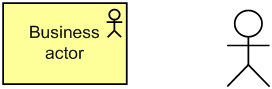
\includegraphics[width=0.3\textwidth]{arquitectura_diseno/imgs/ADMneg1.png} }
		\\ \hline
		Rol de negocio
		&                  
		La responsabilidad de realizar un comportamiento específico, al que se le puede asignar un actor.                                                    &  
		\raisebox{-\totalheight}{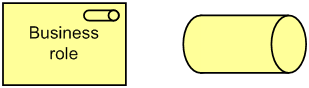
\includegraphics[width=0.3\textwidth]{arquitectura_diseno/imgs/ADMneg2.png} }
		
		\\ \hline
		Colaboración de negocio
		&                  
		
		Un agregado de dos o más negocios
		roles que trabajan juntos para realizar un comportamiento colectivo.                                                    &  
		\raisebox{-\totalheight}{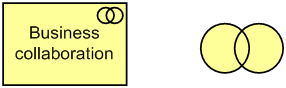
\includegraphics[width=0.3\textwidth]{arquitectura_diseno/imgs/ADMneg3.png} }			 
		
		\\ \hline
		Interfaz de negocio
		&                  
		
		Un punto de acceso donde un servicio comercial está disponible para el medio ambiente.                                                  &  
		\raisebox{-\totalheight}{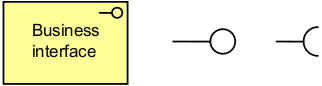
\includegraphics[width=0.3\textwidth]{arquitectura_diseno/imgs/ADMneg4.png} }	
		
		\\ \hline
		Ubicación
		&   Un punto o extensión conceptual en el espacio.                                                                     & \raisebox{-\totalheight}{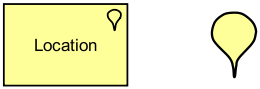
\includegraphics[width=0.3\textwidth]{arquitectura_diseno/imgs/ADMneg5.png} }
		\\ \hline
		Objeto de negocio
		&      
		Un elemento pasivo que tiene relevancia desde una perspectiva empresarial.                                                                  & 
		\raisebox{-\totalheight}{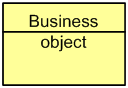
\includegraphics[width=0.3\textwidth]{arquitectura_diseno/imgs/ADMneg11.png} }
		\\ \hline
		
		Proceso de negocio
		&      
		Un elemento de comportamiento que agrupa el comportamiento según un orden de actividades. Su objetivo es producir un conjunto definido de productos o servicios comerciales.                                                                &
		\raisebox{-\totalheight}{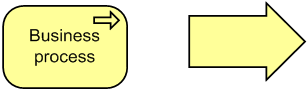
\includegraphics[width=0.3\textwidth]{arquitectura_diseno/imgs/ADMneg6.png} } 
		\\ \hline
		
		Función de negocio
		&      
		
		Un elemento de comportamiento que agrupa el comportamiento en función de un conjunto de criterios elegidos (por lo general, se requieren recursos comerciales y / o competencias).                                                               &
		\raisebox{-\totalheight}{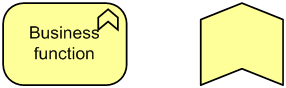
\includegraphics[width=0.3\textwidth]{arquitectura_diseno/imgs/ADMneg7.png} } 
		
		\\ \hline
	\end{tabular}

\begin{tabular}{|c | p{5cm} |  p{5cm}|}
\\ \hline
		Interacción del negocio
		&      
		Un elemento de comportamiento que describe el comportamiento de una colaboración empresarial.                                                              &
		\raisebox{-\totalheight}{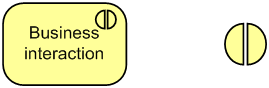
\includegraphics[width=0.3\textwidth]{arquitectura_diseno/imgs/ADMneg8.png} } 
		\\ \hline		
		Evento del negocio
		&      
		Algo que sucede (internamente o
		externamente) e influye en el comportamiento.                                                        &
		\raisebox{-\totalheight}{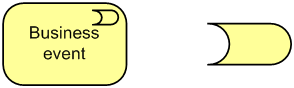
\includegraphics[width=0.3\textwidth]{arquitectura_diseno/imgs/ADMneg9.png} } 
		
		\\ \hline		
		Servicio del negocio
		&      
		Un servicio que satisface las necesidades comerciales de un cliente (interno o externo a la organización).                                                      &
		\raisebox{-\totalheight}{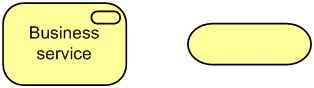
\includegraphics[width=0.3\textwidth]{arquitectura_diseno/imgs/ADMneg10.png} } 		
		
		\\ \hline		
		Representación
		&      
		
		Una forma perceptible de la información transportada por un objeto comercial.                                                     &
		\raisebox{-\totalheight}{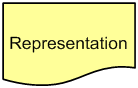
\includegraphics[width=0.3\textwidth]{arquitectura_diseno/imgs/ADMneg12.png} } 
		
		\\ \hline		
		Significado
		&      
		
		
		El conocimiento o experiencia presente en un objeto de negocio o su representación, dado un contexto particular.                                                    &
		\raisebox{-\totalheight}{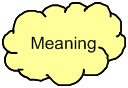
\includegraphics[width=0.3\textwidth]{arquitectura_diseno/imgs/ADMneg13.png} }
		
		\\ \hline		
		Valor
		&      
		
		
		
		El valor relativo, la utilidad o la importancia de un servicio o producto comercial.                                                   &
		\raisebox{-\totalheight}{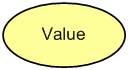
\includegraphics[width=0.3\textwidth]{arquitectura_diseno/imgs/ADMneg14.png} }	
		
		\\ \hline		
		Producto
		&      
		
		Una colección coherente de servicios,
		acompañado de un contrato / conjunto de acuerdos, que se ofrece en conjunto a clientes (internos o externos).                                        &
		\raisebox{-\totalheight}{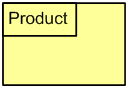
\includegraphics[width=0.3\textwidth]{arquitectura_diseno/imgs/ADMneg15.png} }	
		
		\\ \hline		
		Contrato
		&      
		Una especificación formal o informal de acuerdo que especifica los derechos y obligaciones asociados con un producto..                                        &
		\raisebox{-\totalheight}{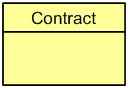
\includegraphics[width=0.3\textwidth]{arquitectura_diseno/imgs/ADMneg16.png} }	
		
		\\ \hline					
	\end{tabular}
\end{center}


\section{Tabla de Aplicación}

\begin{center}
	\begin{tabular}{|c | p{5cm} |  p{5cm}|}
		
		\hline
		Concepto         & Descripción                                                            & Notación
		\\ \hline
		
		Componente de aplicación
		&      
		Una parte modular, implementable y reemplazable de un sistema de software que encapsula su comportamiento y datos y los expone a través de un conjunto de interfaces.                                       &
		\raisebox{-\totalheight}{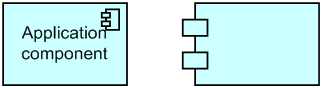
\includegraphics[width=0.3\textwidth]{arquitectura_diseno/imgs/ADMap1.png} }	
		
		\\ \hline		
		
		Colaboración de aplicación
		&      
		
		Un agregado de dos o más componentes de aplicación que trabajan juntos para realizar un comportamiento colectivo.                                      &
		\raisebox{-\totalheight}{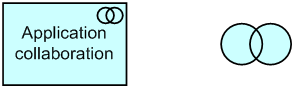
\includegraphics[width=0.3\textwidth]{arquitectura_diseno/imgs/ADMap2.png} }	
		
		\\ \hline		
		
		Interfaz de aplicación
		&      
		
		Un punto de acceso donde un servicio de aplicación está disponible para un usuario u otro componente de aplicación.                                 &
		\raisebox{-\totalheight}{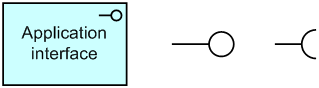
\includegraphics[width=0.3\textwidth]{arquitectura_diseno/imgs/ADMap3.png} }	
		
		\\ \hline		
		
		Objeto de Datos
		&      
		
		
		Un elemento pasivo adecuado para el procesamiento automatizado.                              &
		\raisebox{-\totalheight}{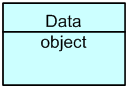
\includegraphics[width=0.3\textwidth]{arquitectura_diseno/imgs/ADMap7.png} }	
		
		
		\\ \hline		
		
		Función de aplicación
		&      
		Un elemento de comportamiento que agrupa el comportamiento automatizado que puede realizar un componente de la aplicación.                             &
		\raisebox{-\totalheight}{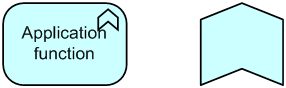
\includegraphics[width=0.3\textwidth]{arquitectura_diseno/imgs/ADMap4.png} }	
		
		\\ \hline		
		
		Interacción de aplicación
		&      
		Un elemento de comportamiento que describe el comportamiento de una colaboración de aplicaciones.                          &
		\raisebox{-\totalheight}{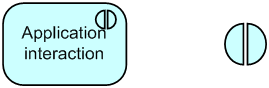
\includegraphics[width=0.3\textwidth]{arquitectura_diseno/imgs/ADMap5.png} }	
		
		\\ \hline		
		
		Servicio de aplicación
		&      
		Un servicio que expone el comportamiento automatizado.                    &
		\raisebox{-\totalheight}{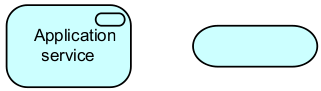
\includegraphics[width=0.3\textwidth]{arquitectura_diseno/imgs/ADMap6.png} }	
		
		\\ \hline		
	\end{tabular}
\end{center}


\section{Tabla de Tecnología}

\begin{center}
	\begin{tabular}{|p{5cm} | p{5cm} |  p{5cm}|}
		
		\hline
		Concepto         & Descripción                                                            & Notación
		\\ \hline
		Nodo & 
		Un recurso computacional sobre el cual los artefactos pueden ser almacenados o desplegados para
		ejecución.&  
		
		\raisebox{-\totalheight}{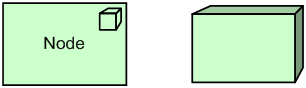
\includegraphics[width=0.3\textwidth]{arquitectura_diseno/imgs/ADMte1.png} }
		\\ \hline
		
		Equipo & 
		Un recurso de hardware sobre el que se pueden almacenar o implementar artefactos para su ejecución.&  
		
		\raisebox{-\totalheight}{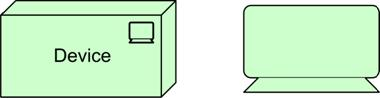
\includegraphics[width=0.3\textwidth]{arquitectura_diseno/imgs/ADMte2.png} }
		\\ \hline
		
		Red & 
		
		Un medio de comunicación entre dos o más dispositivos.&  
		
		\raisebox{-\totalheight}{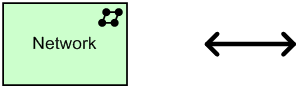
\includegraphics[width=0.3\textwidth]{arquitectura_diseno/imgs/ADMte3.png} }
		\\ \hline
		
		Ruta de comunicación & 
		
		Un enlace entre dos o más nodos, a través del cual estos nodos pueden intercambiar datos.&  
		
		\raisebox{-\totalheight}{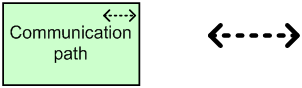
\includegraphics[width=0.3\textwidth]{arquitectura_diseno/imgs/ADMte4.png} }
		\\ \hline
		
		Interfaz de infraestructura & 
		
		Un punto de acceso donde los servicios de infraestructura ofrecidos por un nodo pueden ser accedidos por otros nodos y componentes de la aplicación.&  
		
		\raisebox{-\totalheight}{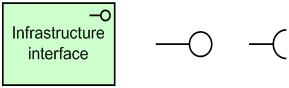
\includegraphics[width=0.3\textwidth]{arquitectura_diseno/imgs/ADMte5.png} }
		\\ \hline
		
		
		Sistema de software & 
		
		Un entorno de software para tipos específicos de componentes y objetos que se implementan en él en forma de artefactos.&  
		
		\raisebox{-\totalheight}{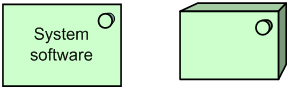
\includegraphics[width=0.3\textwidth]{arquitectura_diseno/imgs/ADMte6.png} }
		\\ \hline
		
		Función de infraestructura & 
		
		Un elemento de comportamiento que agrupa el comportamiento infraestructural que puede realizar un nodo.&  
		
		\raisebox{-\totalheight}{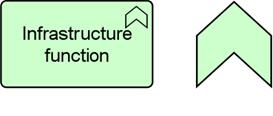
\includegraphics[width=0.3\textwidth]{arquitectura_diseno/imgs/ADMte7.jpg} }
		\\ \hline
		
		Servicio de infraestructura & 
		
		Una unidad de funcionalidad externamente visible, proporcionada por uno o más nodos, expuesta a través de interfaces bien definidas, y
		significativo para el medio ambiente.&  
		
		\raisebox{-\totalheight}{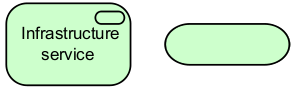
\includegraphics[width=0.3\textwidth]{arquitectura_diseno/imgs/ADMte8.png} }
		
	\end{tabular}
	
	
	\begin{tabular}{|p{5cm} | p{5cm} |  p{5cm}|}
		
		\\ \hline
		
		Artefacto & 
		
		Una pieza física de datos que se usa o
		producido en un proceso de desarrollo de software,
		o por despliegue y operación de un sistema.&  
		
		\raisebox{-\totalheight}{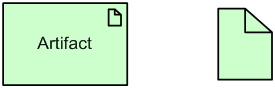
\includegraphics[width=0.3\textwidth]{arquitectura_diseno/imgs/ADMte9.png} }
		\\ \hline
		
	\end{tabular}
\end{center}
\newpage
\section{Tabla de Relaciones}

\begin{center}
	\begin{tabular}{|c | p{5cm} |  p{5cm}|}
		
		\hline
		Relaciones estructurales       && Notación
		\\ \hline
		Asociación & 
		La asociación modela una relación entre objetos que no está cubierta por otra relación más específica.&  
		
		\raisebox{-\totalheight}{
\includegraphics[width=0.3\textwidth]{arquitectura_diseno/imgs/ADMre1.png} }
		\\ \hline
		
		Acceso & 
		La relación de acceso modela el acceso de conceptos de comportamiento a objetos comerciales o de datos.&  
		
		\raisebox{-\totalheight}{
\includegraphics[width=0.3\textwidth]{arquitectura_diseno/imgs/ADMre2.png} }
		\\ \hline		
		
		Usado por & 
		
		La relación utilizada modela el uso de servicios por procesos, funciones o interacciones y el acceso a interfaces por roles, componentes o colaboraciones.&  
		
		\raisebox{-\totalheight}{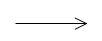
\includegraphics[width=0.3\textwidth]{arquitectura_diseno/imgs/ADMre4.png} }
		\\ \hline		
		
		Realización & 
		
		
		La relación de realización vincula una entidad lógica con una entidad más concreta que la realiza..&  
		
		\raisebox{-\totalheight}{
\includegraphics[width=0.3\textwidth]{arquitectura_diseno/imgs/ADMre5.jpg} }
		\\ \hline		
		
		Asignación & 
		
		La relación de asignación vincula unidades de comportamiento con elementos activos (por ejemplo, roles, componentes) que los realizan o roles con actores que los cumplen.&  
		
		\raisebox{-\totalheight}{
\includegraphics[width=0.3\textwidth]{arquitectura_diseno/imgs/ADMre6.png} }
		\\ \hline		
		
		Agregación & 
		
		
		La relación de agregación indica que un objeto agrupa una cantidad de otros objetos.&  
		
		\raisebox{-\totalheight}{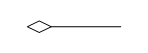
\includegraphics[width=0.3\textwidth]{arquitectura_diseno/imgs/ADMre7.png} }
		\\ \hline		
		
		Composición & 
		
		
		La relación de composición indica que un objeto está compuesto por uno o más objetos diferentes.&  
		
		\raisebox{-\totalheight}{
\includegraphics[width=0.3\textwidth]{arquitectura_diseno/imgs/ADMre8.png} }
		\\ \hline		
		
	\end{tabular}
	\begin{tabular}{|c | p{5cm} |  p{5cm}|}
		\hline
		Relaciones dinamicas && Notación
		\\ \hline
		
		Flujo & 
		La relación de flujo describe el intercambio o transferencia de, por ejemplo, información o valor entre procesos, función,
		interacciones y eventos.&  
		
		\raisebox{-\totalheight}{
\includegraphics[width=0.3\textwidth]{arquitectura_diseno/imgs/ADMre9.png} }
		\\ \hline		
		
		Disparo & 
		
		La relación desencadenante describe las relaciones temporales o causales entre procesos, funciones, interacciones y eventos.&  
		
		\raisebox{-\totalheight}{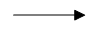
\includegraphics[width=0.3\textwidth]{arquitectura_diseno/imgs/ADMre10.png} }
		\\ \hline		
	\end{tabular}
	
	
	\begin{tabular}{|c | p{5cm} |  p{5cm}|}
		\hline
		Otras relaciones && Notación
		\\ \hline
		
		Agrupación & 
		
		La relación de agrupamiento indica que los objetos, del mismo tipo o diferentes tipos, pertenecen juntos en función de alguna característica común.&  
		
		\raisebox{-\totalheight}{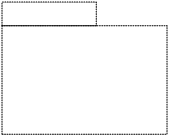
\includegraphics[width=0.3\textwidth]{arquitectura_diseno/imgs/ADMre11.png} }
		\\ \hline		
		
		Unión & 
		
		Un cruce se usa para conectar relaciones del mismo tipo.&  
		
		\raisebox{-\totalheight}{
\includegraphics[width=0.1\textwidth]{arquitectura_diseno/imgs/ADMre12.png} }
		\\ \hline		
		Especialización & 
		
		La relación de especialización indica que un objeto es una especialización de otro objeto.&  
		
		\raisebox{-\totalheight}{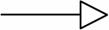
\includegraphics[width=0.1\textwidth]{arquitectura_diseno/imgs/ADMre13.jpg} }
		\\ \hline		
	\end{tabular}
	
\end{center}

\newpage
\section{Tabla de Motivación Migración}

\begin{center}
	\begin{tabular}{|c | p{5cm} |  p{5cm}|}
		\hline
		Concepto & Definición & Notación
		\\ \hline
		
		StakeHolder & 
		
		
		El rol de un individuo, equipo o
		organización (o clases de los mismos) que
		representa sus intereses o preocupaciones en relación con el resultado de la arquitectura..&  
		
		\raisebox{-\totalheight}{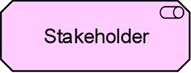
\includegraphics[width=0.3\textwidth]{arquitectura_diseno/imgs/ADMmo1.png} }
		\\ \hline		
		
		Driver & 
		
		Algo que crea, motiva y alimenta el cambio en una organización.&  
		
		\raisebox{-\totalheight}{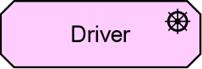
\includegraphics[width=0.3\textwidth]{arquitectura_diseno/imgs/ADMmo2.jpg} }
		\\ \hline		
		
		Assesment & 
		
		El resultado de algún análisis de algún controlador.&  
		
		\raisebox{-\totalheight}{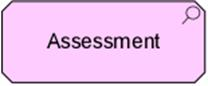
\includegraphics[width=0.3\textwidth]{arquitectura_diseno/imgs/ADMmo3.jpg} }
		\\ \hline		
		
		Meta & 
		
		Un estado final que una parte interesada intenta lograr.&  
		
		\raisebox{-\totalheight}{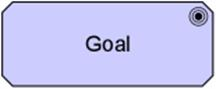
\includegraphics[width=0.3\textwidth]{arquitectura_diseno/imgs/ADMmo4.jpg} }
		\\ \hline		
		
		Requerimiento & 
		
		Una declaración de necesidad que debe ser realizada por un sistema.&  
		
		\raisebox{-\totalheight}{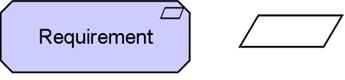
\includegraphics[width=0.4\textwidth]{arquitectura_diseno/imgs/ADMmo5.jpg} }
		\\ \hline		
		
		Restricción & 
		
		Una restricción en la forma en que se realiza un sistema.&  
		
		\raisebox{-\totalheight}{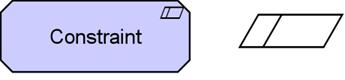
\includegraphics[width=0.4\textwidth]{arquitectura_diseno/imgs/ADMmo6.jpg} }
		\\ \hline		
		
		Principio & 
		
		
		Una propiedad normativa de todos los sistemas en un contexto dado, o la forma en que se realizan.&  
		
		\raisebox{-\totalheight}{\includegraphics[width=0.3 \textwidth]{arquitectura_diseno/imgs/ADMmo7.jpg} }
		\\ \hline		
	\end{tabular}
\end{center}

\newpage


\section{ADM}
contenido...
\begin{figure}[th!]
	\centering
	\includegraphics[width=0.7\linewidth]{arquitectura_diseno/imgs/adm}
	\caption{ADM}
\end{figure}
